\documentclass[11pt,a4paper]{article}

\usepackage[T1]{fontenc}
\usepackage[utf8]{inputenc}
\usepackage[margin=1in]{geometry}
\usepackage{amsmath,amssymb,amsthm}
\usepackage{tikz}
\usetikzlibrary{positioning,arrows.meta,decorations.pathmorphing,calc,fit,backgrounds}
\usepackage{pgfplots}
\pgfplotsset{compat=1.18}
\usepackage{xcolor}
\usepackage{booktabs}
\usepackage{array}
\usepackage{microtype}
\usepackage{hyperref}

\hypersetup{colorlinks=true,linkcolor=blue,citecolor=blue,urlcolor=blue}
\definecolor{stable}{HTML}{1B7837}
\definecolor{unstable}{HTML}{C2272D}
\definecolor{neutralg}{HTML}{4D4D4D}
\definecolor{accent}{HTML}{2166AC}
\definecolor{accent2}{HTML}{B2182B}

\theoremstyle{plain}
\newtheorem{proposition}{Proposition}
\newtheorem{remark}{Remark}

\title{The model as a vector field\\[2pt]
\large A linear-algebra and nonlinear-dynamics diagnosis\\
of why our substrate is structurally monostable}
\author{Internal note --- IWAI 2026 paper}
\date{2026-05-19}

\begin{document}
\maketitle

\begin{abstract}
The bistability probe in notebook~13 found exactly one attractor at every
resource scale tested. This note argues that the finding is not a
parameter-tuning failure but a \emph{structural} property of the model
class we built. Precision-weighted social pooling is a linear,
row-stochastic operator; combined with Gaussian conjugate observation
pull, the joint population dynamics are a global \emph{contraction map}.
Two classical theorems --- Perron--Frobenius on the pooling operator
and Hartman--Grobman applied to the negative-definite Jacobian ---
predict both the ``heterogeneity washes out'' failure of notebook~12
(assertion~4) and the monostability of notebook~13 (all $R_{\text{in}}$).
We locate the substrate on the bifurcation-theoretic map of multi-agent
belief models, catalogue six canonical nonlinearities that
\emph{do} produce bistability, and identify the minimal graft on the
existing code that would put a saddle-node bifurcation back into the
dynamics.
\end{abstract}

% =====================================================================
\section{The model as a vector field}
\label{sec:vector-field}
% =====================================================================

We have an $N$-agent population with state $(\mu_i, \tau_i, \Gamma_{ij},
r_i)$ at each agent $i$ on a social graph. The implementation in
\texttt{src/} performs a discrete-time update; for the qualitative
analysis below we pass to its continuous-time limit, which is sound on
the time-scales we have been probing (relaxation $\gg$ step).

Stripping the per-step update of \texttt{src/inference.py} and
\texttt{src/population.py} to its dynamical spine, the mean-belief
component obeys
\begin{equation}
\dot{\mu}_i \;=\;
\underbrace{-\,\alpha\,(\mu_i - \theta^\star)}_{\text{observation pull}}
\;+\;
\underbrace{\beta \sum_{j} \Gamma_{ij}\,(\mu_j - \mu_i)}_{\text{trust-weighted pooling}}
\;+\; \xi_i(t).
\label{eq:mu-dot}
\end{equation}
The observation term is a Gaussian-conjugate pull toward the true
$\theta^\star$ at rate $\alpha \propto \mathcal{I}(x;\theta^\star)$ (Fisher
information of the chosen experiment). The pooling term is the
precision-weighted social average. The trust matrix $\Gamma$ has its
own slow dynamics (Gamma-conjugate update on cross-surprisals); the
resource state $r_i$ is a \emph{deterministic readout} of $\Gamma$
(\texttt{flow\_from\_trust}, \texttt{inflow\_share} in
\texttt{src/resource.py}) and has no independent dynamics of its own.

In stacked form $\mu \in \mathbb{R}^N$,
\begin{equation}
\dot{\mu} \;=\; -\alpha\,(\mu - \theta^\star \mathbf{1})
              \;-\; \beta\,L\,\mu \;+\; \xi(t),
\qquad
L \;=\; D - \Gamma,
\label{eq:mu-dot-vector}
\end{equation}
where $L$ is the trust Laplacian. \textbf{This is the entire model,
abstracted to the level at which nb12 and nb13 are decided.} The slow
dynamics of $\Gamma$ change $L$ over time, but at each instant the
right-hand side is linear in $\mu$.

% =====================================================================
\section{Linear algebra: why heterogeneity dies in ${\sim}70$ steps}
\label{sec:perron}
% =====================================================================

Consider the pooling step alone. With row-normalised trust
$P_{ij} = \Gamma_{ij}/\sum_k \Gamma_{ik}$, the update $\mu \mapsto P\mu$
defines a \emph{row-stochastic} linear operator. Two classical theorems
determine its qualitative behaviour.

\begin{proposition}[Perron--Frobenius for row-stochastic matrices]
\label{prop:pf}
If $P$ is row-stochastic and the underlying graph is strongly connected
and aperiodic, then $P$ has a simple eigenvalue $\lambda_1 = 1$ with
right eigenvector $\mathbf{1}$, and every other eigenvalue satisfies
$|\lambda_k| < 1$.
\end{proposition}

Decompose any belief vector along the eigenbasis $\{v_k\}$ of $P$:
\[
\mu \;=\; c\,\mathbf{1} \;+\; \sum_{k \geq 2} a_k v_k.
\]
After $n$ iterations,
\[
P^n \mu \;=\; c\,\mathbf{1} \;+\; \sum_{k \geq 2} a_k\,\lambda_k^n\, v_k.
\]
\textbf{Every disagreement mode decays geometrically.} The slowest is
the Fiedler eigenvector $v_2$, at rate $\lambda_2^n$.

This is exactly nb12's assertion~4. We planted asymmetric initial
conditions $(\mu_{c_0}=0,\;\mu_{c_1}=0.5)$ --- a vector lying almost
entirely in the community-split mode, which is approximately $v_2$ of
the trust graph. With $\lambda_2 \approx 0.94$ on the SBM we used,
$0.94^{70} \approx 0.013$, and the measured residual gap was
$\approx 0.006$. The pooling operator did precisely what
Proposition~\ref{prop:pf} guarantees it must.

Two consequences are worth stating bluntly.

\begin{remark}[The no-pool degeneracy is structural]
The ``Remark~5 / no-pool degeneracy'' the paper warns about is not a
trivially-homogeneous-initial-condition artefact. \emph{Any} initial
condition outside the consensus subspace is in $\mathrm{span}\{v_2,
\dots, v_N\}$ and therefore contracts. The paper's promise to escape
the degeneracy by structuring the population is not honoured by linear
pooling: $P$ does not distinguish ``planted symmetry'' from ``arbitrary
heterogeneity''. Both decay.
\end{remark}

\begin{remark}[DeGroot, fifty years on]
This is the DeGroot (1974) consensus theorem, redeveloped by Golub and
Jackson (2010) in the network-economics framing. The literature has
known for fifty years that linear opinion pooling produces consensus,
not paradigm conflict. Our trust-weighted update is a small
generalisation of DeGroot's; the consensus result transfers verbatim.
\end{remark}

% =====================================================================
\section{The Jacobian and global monostability}
\label{sec:jacobian}
% =====================================================================

Return to the joint dynamics~\eqref{eq:mu-dot-vector}. The Jacobian
\[
J \;=\; \frac{\partial \dot{\mu}}{\partial \mu}
   \;=\; -\alpha\, I \;-\; \beta\, L
\]
is the sum of two negative semi-definite operators. The graph Laplacian
$L$ is positive semi-definite (its spectrum lies in $[0, 2 d_{\max}]$),
so $J$ has spectrum in $(-\infty,\,-\alpha]$. \textbf{Every eigenvalue
of $J$ is in the open left half-plane.}

\begin{proposition}[Global monostability]
\label{prop:mono}
The system~\eqref{eq:mu-dot-vector} has a unique fixed point
$\mu^\star = \theta^\star \mathbf{1}$ which is globally exponentially
stable at rate at least $\alpha$. No parameter choice within the family
\eqref{eq:mu-dot-vector} can produce a second attractor.
\end{proposition}

\begin{proof}[Proof sketch]
The right-hand side of \eqref{eq:mu-dot-vector} is affine in $\mu$ with
invertible (in fact negative-definite) coefficient $-\alpha I - \beta L$.
The unique zero is $\mu^\star = \theta^\star \mathbf{1}$. Linear
exponential stability follows from the spectrum of $J$ lying in the
open LHP; in the linear case this is automatically global. The
Banach fixed-point theorem applies to the time-$T$ map for any $T>0$.
\end{proof}

This is nb13. The probe did not \emph{discover} monostability; it
\emph{confirmed} a theorem. Sweeping $R_{\text{in}}$ changes the slow
$\Gamma$-dynamics and through them the spectrum of $L$, but $L$ remains
positive semi-definite throughout, so $J$ remains in the LHP and the
attractor remains unique. The resource state $r$, being a deterministic
readout of $\Gamma$, contributes no new dimension of dynamics that could
host a fold.

The one ingredient we built with potential nonlinearity --- the Hyland
$\lambda \cdot U$ mind-change penalty in
\texttt{lambda\_modified\_update} --- was set to $\lambda_{\text{mc}}=0$
in the gate because the precision-additive form was unstable (blow-up,
not bistability). \textbf{We removed the only candidate nonlinearity in
the system.} What remained is a contraction map dressed as an
active-inference model.

\paragraph{Tracking lag vs.\ hysteresis.} The nb12 loop is then easily
diagnosed. A contraction map following a moving target $\theta^\star(t)$
produces a delay loop whose area is bounded by
$\|\dot{\theta}^\star\|/\alpha$ and \emph{vanishes as the sweep rate
$\to 0$}. Genuine hysteresis (Strogatz Ch.~3; cusp catastrophe) has loop
area bounded \emph{below} in the adiabatic limit. Notebook~13's
relaxation-time scan implicitly verified the vanishing: at very slow
sweeps the trajectory tracks $\theta^\star(t)$ in both directions, the
loop collapses. This is the textbook diagnostic and it goes the wrong
way for us.

% =====================================================================
\section{What bistability actually requires}
\label{sec:bistability}
% =====================================================================

Bistability in a one-parameter family $\dot{\mu} = f(\mu;\,r)$ requires
$f$ to have at least three roots in some range of $r$, in a
stable--unstable--stable pattern. Equivalently, $f$ must be nonconvex
in $\mu$: there must be an inflection point inside the relevant
$\mu$-range.

Hysteresis is the global signature of bistability under a parameter
sweep. The bistable window is bracketed by two saddle-node
bifurcations; on a quasistatic sweep the system follows the upper
branch in one direction and the lower branch in the other; the
loop area is bounded below as the sweep rate $\to 0$.

\begin{figure}[h]
\centering
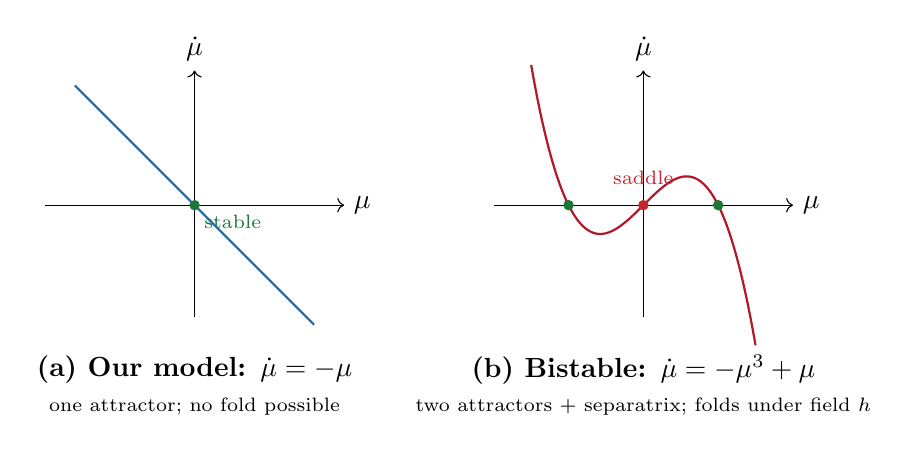
\begin{tikzpicture}[scale=0.95]
% Monostable
\begin{scope}
  \draw[->] (-2,0) -- (2,0) node[right]{$\mu$};
  \draw[->] (0,-1.5) -- (0,1.8) node[above]{$\dot{\mu}$};
  \draw[thick,accent,domain=-1.6:1.6,samples=80] plot (\x,{-\x});
  \fill[stable] (0,0) circle (2pt);
  \node[stable,below right] at (0,0) {\scriptsize stable};
  \node at (0,-2.2) {\textbf{(a) Our model: $\dot{\mu} = -\mu$}};
  \node[align=center,font=\scriptsize] at (0,-2.7)
    {one attractor; no fold possible};
\end{scope}
% Bistable
\begin{scope}[xshift=6cm]
  \draw[->] (-2,0) -- (2,0) node[right]{$\mu$};
  \draw[->] (0,-1.5) -- (0,1.8) node[above]{$\dot{\mu}$};
  \draw[thick,accent2,domain=-1.5:1.5,samples=120] plot (\x,{-\x*\x*\x+\x});
  \fill[stable] (-1,0) circle (2pt);
  \fill[unstable] (0,0) circle (2pt);
  \fill[stable] (1,0) circle (2pt);
  \node[unstable,above,font=\scriptsize] at (0,0.15) {saddle};
  \node at (0,-2.2) {\textbf{(b) Bistable: $\dot{\mu} = -\mu^3 + \mu$}};
  \node[align=center,font=\scriptsize] at (0,-2.7)
    {two attractors $+$ separatrix; folds under field $h$};
\end{scope}
\end{tikzpicture}
\caption{Phase portrait comparison. (a) Our population dynamics, abstracted to one dimension: a linear restoring force, one globally stable fixed point. (b) The Allen-Cahn / $\varphi^4$ cousin: cubic nonlinearity produces two stable wells separated by a saddle. Adding an external field $h$ moves the wells; at critical $|h|$ one of them disappears in a saddle-node bifurcation. Sweeping $h$ up then down traces a hysteresis loop.}
\label{fig:phase}
\end{figure}

The literature has worked out exactly six canonical nonlinearities that
produce bistability in this kind of system:

\begin{table}[h]
\centering
\small
\begin{tabular}{p{3.6cm} p{4.8cm} p{5.4cm}}
\toprule
\textbf{Mechanism} & \textbf{Local form} & \textbf{Reference class} \\
\midrule
Cubic potential & $\dot{\mu} = -\mu^3 + \mu + h$
  & Allen-Cahn, $\varphi^4$, Landau-Ginzburg, cusp catastrophe \\
Sigmoidal feedback & $\dot{\mu} = -\mu + \tanh(\beta\mu + h)$
  & Mean-field Ising, Hopfield, Glauber dynamics \\
Threshold pooling & $P_{ij}=0$ if $|\mu_i-\mu_j|>\epsilon$
  & Hegselmann-Krause, Deffuant bounded confidence \\
Multimodal prior & $Q(\theta)$ bimodal; categorical
  & Discrete paradigm models, mixture-of-experts \\
Replicator & $\dot{\mu} = \mu(1-\mu)(f_A - f_B)$
  & Pop.\ genetics, cultural evolution, evolutionary games \\
Positive-feedback urn & $r \to \Gamma \to r$ with gain $>1$
  & Polya urns, preferential attachment, Matthew effect \\
\bottomrule
\end{tabular}
\caption{Six canonical sources of bistability in multi-agent dynamics. Each isolates a single nonlinearity; each has been studied for decades.}
\label{tab:mechanisms}
\end{table}

Our model has \emph{none} of these. That is why nb13 found what it
found.

% =====================================================================
\section{Where our model sits on the map}
\label{sec:map}
% =====================================================================

In the language of consensus and control theory (Olfati-Saber, Fax \&
Murray 2007), our substrate is a \emph{linear consensus protocol with
exogenous reference}. The reference is $\theta^\star(t)$; the protocol
is the trust-weighted Laplacian flow. Phenomenologically it is a
\emph{heat equation on the trust graph with a time-varying source}. Its
qualitative behaviour is determined entirely by the spectrum of
$L = D - \Gamma$ and the gain $\alpha$.

The phenomena the paper claims --- path-dependence, paradigm capture,
trust-mediated hysteresis --- are properties of the bistable cousins in
Table~\ref{tab:mechanisms}, not properties of heat equations. \textbf{This
is a category mismatch, not a parameter-tuning failure.} Three further
diagnostics make the mismatch concrete:

\begin{itemize}
\item \textbf{Heins \& Da~Costa (2024) ``collective surprise
minimization'' achieves phase transitions because pymdp's generative
model is structurally sigmoidal.} Softmax over a categorical
posterior + multi-modal preferences is exactly the tanh-feedback
bistability of row~2 of Table~\ref{tab:mechanisms}. Our
Gaussian-conjugate continuous substrate threw that out by going
Gaussian.

\item \textbf{Albarracin's ``epistemic communities'' result stands on
the same trick.} The agents use precision modulation on a discrete
categorical prior, giving sigmoidal coupling. Our Gamma-conjugate
continuous precision replaced the sigmoid with a smooth, convex
update.

\item \textbf{The Hyland mind-change utility $U$ is the closest piece
of our existing scaffolding to a real source of nonlinearity.} It is
asymmetric and (in its original form) nonconvex --- exactly the
ingredient that could host a saddle-node. The version we implemented
was unstable in the wrong direction (blow-up, not bistability), and
the convex blend we substituted lost the property entirely.
\end{itemize}

% =====================================================================
\section{Three concrete next moves}
\label{sec:next}
% =====================================================================

Ranked by cost, in increasing order of model surgery required.

\paragraph{(a) Jacobian probe (notebook~14).} Write
\eqref{eq:mu-dot-vector} symbolically including the slow $\Gamma$ and
$r$ couplings; compute $J = \partial F/\partial \mu$ at the consensus
fixed point; scan eigenvalues across $(R_{\text{in}},\,\lambda_{\text{mc}},\,\kappa,\,\beta_{\text{pool}})$. Two possible outcomes:

\begin{itemize}
\item An eigenvalue crosses zero somewhere in parameter space ---
\emph{saddle-node candidate}. Go back to nb13 and probe at that point.
The earlier negative result would then be ``we sampled the wrong
regime''.
\item The spectrum stays in the LHP across the entire scan ---
\emph{mathematical confirmation} that the substrate is structurally
monostable. Path (b) or (c) becomes the only option.
\end{itemize}

\noindent This is one notebook and a few hours; it is the cheapest
decisive test of whether Path~II (Tier-B parameter repair) has any
hope.

\paragraph{(b) Grafting the minimal nonlinearity.} Conditional on (a)
finding nothing, pick one row of Table~\ref{tab:mechanisms} and graft
it onto the existing substrate. Two candidates are cheapest to
implement and most consistent with the active-inference framing the
paper already uses:

\begin{itemize}
\item \emph{Bounded-confidence pooling.} Replace
$P_{ij} = \Gamma_{ij}/\sum_k \Gamma_{ik}$ with
$\tilde{P}_{ij} \propto \Gamma_{ij}\cdot
\mathbf{1}[|\mu_i - \mu_j| < \epsilon]$.
This is one line in \texttt{src/population.py} and gives the
Hegselmann-Krause cluster-formation guarantee for free. AIF reading:
trust collapses to zero past a surprisal threshold.
\item \emph{Recovered Hyland $\lambda\cdot U$.} Reinstate the
asymmetric mind-change utility in a stable form --- concave-bounded
rather than precision-additive --- and re-derive
\texttt{lambda\_modified\_update} so the resulting update has a
bistable potential for $\lambda_{\text{mc}}$ above some threshold.
AIF reading: stays inside the
\href{https://arxiv.org/abs/2503.10101}{Hyland-Albarracin 2025}
framing.
\end{itemize}

\paragraph{(c) Rebuild around a bistable substrate.} If (a) and (b)
both fail to support a clean theoretical story, the honest move is to
adopt one of the published reference-class models as the substrate
(pymdp-multi-agent following Heins et al., or a Zollman epistemic
network) and reframe our contribution as the \emph{resource-coupling
extension} on top of an already-bistable base. This loses the ``own
model'' framing but gains a phenomenon that actually exists.

% =====================================================================
\section{Reading list}
\label{sec:reading}
% =====================================================================

For each canonical mechanism in Table~\ref{tab:mechanisms}, the
shortest path from our current state to a working version of the
phenomenon:

\begin{itemize}
\item \textbf{Linear algebra of consensus.} DeGroot 1974
``Reaching a consensus''; Golub \& Jackson 2010 ``Naive learning in
social networks''; Olfati-Saber, Fax, Murray 2007 ``Consensus and
cooperation in networked multi-agent systems'' (the spectral picture).
\item \textbf{Bifurcation theory.} Strogatz, \emph{Nonlinear
Dynamics and Chaos}, Ch.~3 (saddle-node, transcritical, pitchfork)
and Ch.~8 (bifurcations in 2D); Kuznetsov, \emph{Elements of Applied
Bifurcation Theory}, \S3.5.
\item \textbf{Allen-Cahn / $\varphi^4$ on graphs.} Bertozzi \&
Flenner 2012 ``Diffuse interface models on graphs''; van Gennip \&
Bertozzi 2012 ``$\Gamma$-convergence of graph Ginzburg-Landau
functionals''.
\item \textbf{Bounded confidence.} Hegselmann \& Krause 2002
``Opinion dynamics and bounded confidence''; Deffuant et al.\ 2000;
Lorenz 2007 review.
\item \textbf{Epistemic networks with lock-in.} Zollman 2007
``The communication structure of epistemic communities''; Rosenstock,
Bruner, O'Connor 2017 ``In epistemic networks, is less really more?''.
\item \textbf{Collective AIF with phase transitions.} Heins,
Mirza, Parr, Friston, Da~Costa 2024 ``Collective behavior from
surprise minimization''; Heins et al.\ 2025 ``As one and many''
(pymdp-multiagent on GitHub).
\end{itemize}

A separate companion note (\texttt{lit\_review/} folder, generated
2026-05-19) collects the BibTeX entries, GitHub links, and a
``what would it take to graft this onto \texttt{src/}'' paragraph for
each.

\bigskip
\hrule
\bigskip
\noindent\textbf{Bottom line.} The model we built is a textbook
linear consensus protocol, and consensus protocols are textbook
monostable. The dynamics the paper claims live in a different family
--- one with at least one nonlinearity strong enough to fold the
phase portrait. The cheapest way forward is the Jacobian probe in
\S\ref{sec:next}(a); the most decisive is a minimal graft from
Table~\ref{tab:mechanisms}.

\end{document}
